\begin{frame}{El concepto de convexidad.}
  \Defi{*}{
    Sea $X$ un espacio normado y $H\subseteq X$ un conjunto no vacío.
    Decimos que el conjunto $H$ es \emph{convexo\footnotemark}, si \alert{para todo}
    par de elementos $x,y \in H$, se tiene que el segmento
    de recta que los une
    \Eq{segment}{
      [x,y] := \{tx + (1-t)y \quad |\quad t\in[0,1]\}
    }
    está, contenido en $H$, i.e., $[x,y]\subseteq H$.
  }
  \begin{figure}
    \centering
    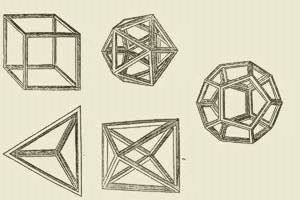
\includegraphics[scale=0.3]{images/davinciplatonic.jpg}
    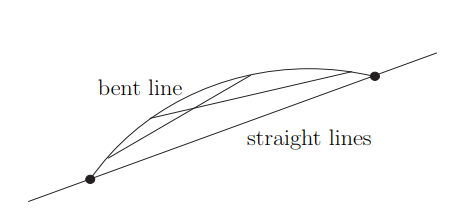
\includegraphics[scale=0.3]{images/convexity_by_archimides.png}
    \caption{Cinco s\'olidos plat\'onicos y la convexidad según Arquímides.}
  \end{figure}
  \footnotetext[1]{
    Hay en un plano ciertas líneas,
    que o bien se encuentran totalmente en el mismo lado 
    de las líneas rectas que unen sus extremidades,
    O no tienen parte de ellos en el otro lado.
    Archimedes of Syracuse (Sicily), ca 287 - ca 212 B.C.
    On the sphere and cylinder \alert{(Incluir referencia)}
  }
\end{frame}